\documentclass{article}
\usepackage[utf8]{inputenc}
\usepackage[greek,english]{babel}
\usepackage{alphabeta}
\usepackage{fancyhdr}
\usepackage{listings}
\usepackage{mathtools}
\usepackage{xcolor}
\usepackage{biblatex}
\usepackage[left=1cm,right=1cm]{geometry}

\lstset {
        basicstyle=\ttfamily,
        columns=fullflexible,
        breaklines=true,
        keepspaces=true,
	showstringspaces=false
}

\title{Εργαστήριο Κατανεμημένων Συστημάτων - Εργασία 2}
\author{Χρήστος Μαργιώλης -- 19390133}
\date{Μάιος 2022}

\begin{document}

\begin{titlepage}
        \maketitle
        \begin{figure}[t!]
        \begin{center}
        
\includegraphics[scale=0.3]{./res/uniwalogo.png} \\
        \Large
        \textbf{Πανεπιστήμιο Δυτικής Αττικής} \\
        \large
        Τμήμα Μηχανικών Πληροφορικής και Ηλεκτρονικών Υπολογιστών
        \end{center}
        \end{figure}
\end{titlepage}

\renewcommand{\contentsname}{Περιεχόμενα}
\tableofcontents

\section{Δομή αρχείων}

\begin{itemize}
	\item \lstinline{HRInterface}: Interface που περιέχει τις δηλώσεις των
		μεθόδων του server.
	\item \lstinline{HRImpl}: Υλοποίηση του interface.
	\item \lstinline{Room}: Βοηθητική κλάση για την υλοποίηση των δωματίων
		του ξενοδοχείου.
	\item \lstinline{HRServer}: Ο server.
	\item \lstinline{HRClient}: Ο client.
\end{itemize}

\section{Εκτέλεση κώδικα}

Κάνουμε compile τον κώδικα:

\begin{lstlisting}
	$ javac *.java
\end{lstlisting}

Ανοίγουμε δύο terminals. Στο ένα ξεκινάμε το \lstinline{rmiregistry} και στο
άλλο τον server. Σε τρίτο terminal εκτελούμε τον client, ο οποίος μπορεί
να εκτελεστεί με έναν από τους 4 τρόπους:

\begin{lstlisting}
	java HRClient list <hostname>
	java HRClient book <type> <number> <name> <hostname>
	java HRClient guests <hostname>
	java HRClient cancel <type> <number> <name> <hostname>
\end{lstlisting}

\section{Ενδεικτικά τρεξίματα}

Τα παρακάτω τρεξίματα δείχνουν τους 4 διαφορετικούς τρόπους εκτέλεσης του
client, καθώς και τους χειρισμούς περιπτώσεων που μπορούν να προκείψουν (π.χ
δεν υπάρχουν ελεύθερα δωμάτια, υπάρχουν λιγότερα δωμάτια από όσα θέλει να
κρατήσει ο πελάτης)

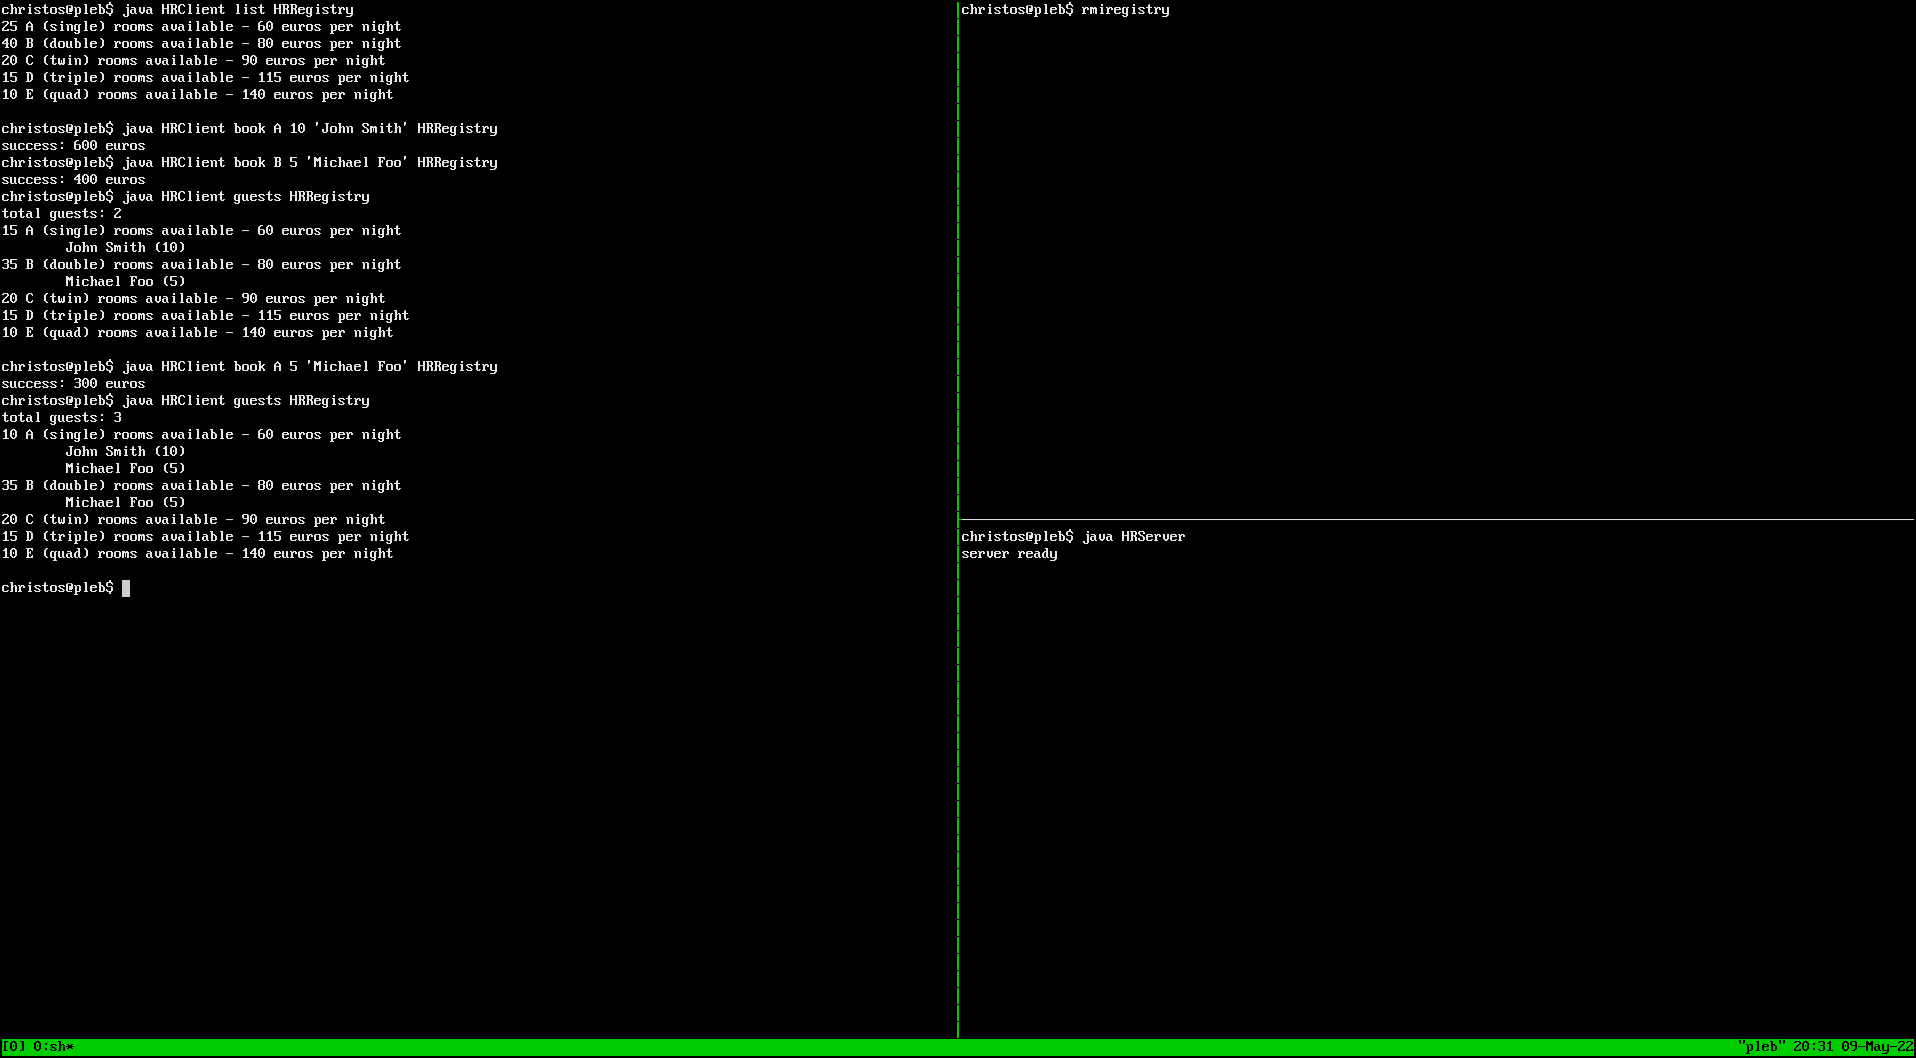
\includegraphics[width=\linewidth]{res/run1.png}
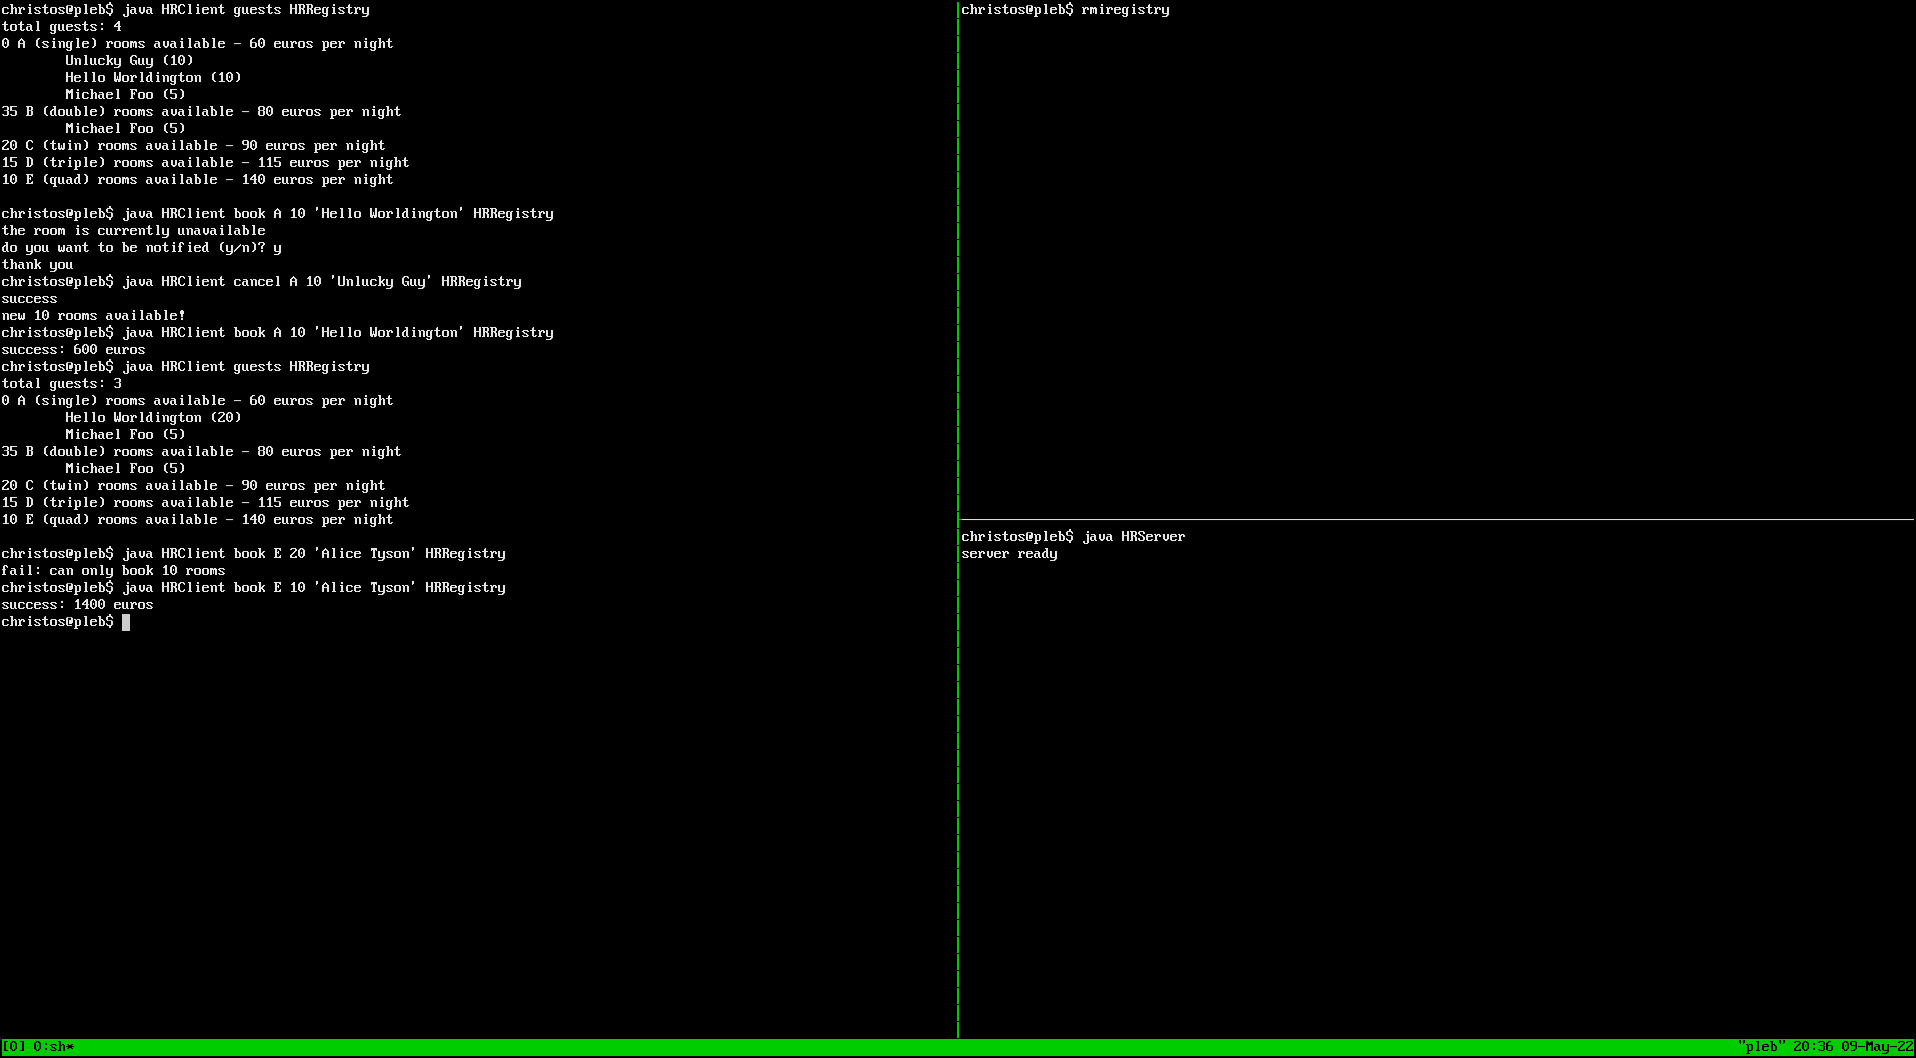
\includegraphics[width=\linewidth]{res/run2.png}

\section{Κώδικας}

Ο κώδικας είναι σχολιασμένος στα σημεία που θεωρώ ότι μπορεί να υπάρξει
σύχγηση, και όχι ακόμα και σε σημεία που είναι λίγο-πολύ ξεκάθαρο το τι
συμβαίνει.

\subsection{\lstinline{HRInterface.java}}

\lstinputlisting[language=java]{../src/HRInterface.java}
\pagebreak

\subsection{\lstinline{HRImpl.java}}

\lstinputlisting[language=java]{../src/HRImpl.java}
\pagebreak

\subsection{\lstinline{Room.java}}

\lstinputlisting[language=java]{../src/Room.java}
\pagebreak

\subsection{\lstinline{HRServer.java}}

\lstinputlisting[language=java]{../src/HRServer.java}
\pagebreak

\subsection{\lstinline{HRClient.java}}

\lstinputlisting[language=java]{../src/HRClient.java}
\pagebreak

\end{document}
